% !TEX root = ./main.tex
\chapter{Introduction}

This chapter discusses fundamental properties of aerosols and computational modeling techniques which motivate this thesis. A description of atmospheric aerosols and the challenges associated with capturing the complexity of aerosol properties and their environmental feedbacks is discussed. Additionally, numerical modeling treatments for aerosols are presented along with approaches to improve the characterization of aerosol complexity. Finally, research questions are presented which outline primary avenues of inquiry for this thesis.  

\section{The complexity of aerosols and environmental feedbacks}\label{aerosol_properties}

An aerosol is a collection of particles composed of one or more chemical species that are suspended in a fluid or gas. In the atmosphere, aerosol particles vary considerably in terms of their physical properties such as size, composition, and origin. Additionally, the chemical, thermodynamic, and radiative properties of aerosol particles can alter the state of the aerosol and the surrounding environment through numerous feedback mechanisms. In turn, aerosol particles exhibit a complex, non-linear coupling with the environment that spans broad spatial and temporal scales.

Aerosol particles are typically measured by their diameter where spherical morphology is assumed. The smallest particles have diameters on the order of 1 nm and are produced via the nucleation of low-volatility vapors. On the opposite extreme of particle sizes, the largest particle diameters can exceed 100 $\upmu$m. In total, aerosols span approximately five orders of magnitude. To capture the broad scale of particle diameters that may be present in a population of aerosol particles, aerosol size distributions often represent the number concentration of particles as a function of the logarithm of particle diameter. The particle size distribution may be represented by multiple modes---lognormal size distributions---that are differentiated by the characteristics of particles within each mode, including growth and removal mechanisms. Typically, three distinct modes are present in a particle size distribution: the nucleation, accumulation, and coarse mode. 

Nucleation mode particles are up to 20 nm in diameter and undergo rapid growth as gas-phase species condense onto the particle surface or as particles inelastically collide through coagulation. They are removed from the nucleation mode by growth within \hl{XX} time into the accumulation mode, which spans particle diameters from 0.1 $\upmu$m to 2 $\upmu$m . In addition to particles that enter the accumulation mode through growth by condensation or coagulation, particles may be released directly into the accumulation mode via primary emissions. Removal mechanisms such as wet and dry deposition are least efficient in the accumulation mode, allowing particles to remain suspended in the atmosphere for days to weeks. Particles in the coarse mode have diameters exceeding 2 $\upmu$m  and are produced by mechanical processes such as abrasion and the resuspension of dust. Due to their size, particles in the coarse mode are rapidly removed by gravitational settling within minutes to hours. This multi-modal description of the aerosol size distribution points to the inherent complexity of aerosol population dynamics---production, growth, and removal mechanisms differ considerably by particle size. 

As noted, production mechanisms vary across aerosol modes (e.g., nucleation of low-volatility vapors, emission of primary aerosol  into the accumulation mode, resuspension of coarse particles, etc.). These processes typically involve different chemical species. For example, whereas volatile organic compounds (VOCs) such as isoprene and other organic carbon (OC) species may undergo oxidation reactions which lower their volatility and promote particle nucleation, particles released directly into the accumulation or coarse mode as primary aerosol may consist of either organics that are produced during combustion such as black carbon (BC) or inorganics such as sea salt spray, mineral dust, \hl{[other species]}. \hl{Here its worth acknowledging contribution of precursor emissions to chemical aging, secondary production of aerosol-phase matter, changes to aerosol mixing state, etc.}. As a result, aerosol particles are compositionally diverse. 

In addition to diversity in the composition of aerosol particles across the size distribution, aerosol populations also exhibit spatiotemporal variations which alter the local structure and composition of the aerosol. The geographic distribution of emission sources, varied land use, and topography lead to spatial heterogeneities in the emission of gas-phase precursors and primary aerosols. Additionally, temporal trends alter the meteorological state of the atmosphere and the concentration of reactive gas or aerosol-phase species. For instance, diurnal variation in the structure of the boundary layer due to surface heating determines the strength of vertical transport and mixing of primary aerosol or reactive gas-phase species. \hl{[Could talk about photolysis]}. Furthermore, the timing of emissions may play a crucial role in determining whether a chemical reaction will take place; reactive species must be present in the same space and time to undergo reaction.

\cite{seinfeld_atmospheric_1998}

\section{Impacts of aerosols on climate}

Aerosols alter the Earth's radiative budget directly through scattering and absorption of shortwave (solar) radiation. The scattering of solar radiation by aerosols back out to space increases planetary albedo, thereby decreasing the intensity of radiation reaching the Earth's surface (\cite{charlson_climate_1969}; \cite{charlson_climate_1992}). As a result, scattering generally contributes a net cooling effect. The intensity of scattering depends on the composition of the aerosol, with strongly-scattering species including sulfate and nitrate. Aerosols may also absorb broadband radiation, re-emitting in the form of thermal radiation that results in a net warming effect. Absorption varies by aerosol species; strongly absorbing species include carbonaceous aerosol such as black carbon and elemental carbon. Scattering and absorption of solar radiation due to aerosols alters the stability of the atmosphere due to changes in the vertical profile of temperature (\cite{li_scattering_2022}; \cite{lau_observational_2006}). 

In addition to direct aerosol-radiative effects, aerosols also alter the climate through indirect effects with clouds commonly referred to as aerosol-cloud interactions. Hygroscopic aerosol particles act as cloud condensation nuclei (CCN), thereby allowing water vapor to condense onto their surface at ambient supersaturations $S$ typical of the troposphere ($S\lesssim1\%$). \cite{twomey_influence_1977} was the first to note that higher concentrations of CCN result in a greater abundance of small cloud droplets. This in turn leads to an increase in cloud albedo, causing greater reflection of solar radiation back to space and thus a net cooling effect on climate. In addition to the Twomey effect, the impact of aerosol number concentration on droplet size can delay or prevent the onset of collision-coalescence necessary to initiate precipitation. This effect was first discovered by \cite{albrecht_aerosols_1989} and enhances the lifetime of clouds, thereby prolonging the reflection of solar radiation. 

The global mean effective radiative forcing (ERF) due to the combination of direct and indirect effects is estimated by the Intergovernmental Panel on Climate Change (IPCC) to be in the range of -2.0 to -0.6 \si{W.m^{-2}} within 95\% confidence, with a mean of -1.3 \si{W.m^{-2}} (\cite{ipcc_report_2021}). Separating the ERF into forcing due to aerosol-cloud interactions and direct radiative forcing, aerosol-cloud interactions contribute the largest magnitude of forcing in the range -1.7 to -0.3 \si{W.m^{-2}} with a mean of -1.0 \si{W.m^{-2}}. Direct effects contribute -0.6 to 0.0 \si{W.m^{-2}} with a mean of -0.3 \si{W.m^{-2}}. 

The magnitude of uncertainty in ERF due to aerosol direct and indirect effects remains large due to a host of factors. As discussed in Section \ref{aerosol_properties}, aerosol particle size and composition are highly varied and determine climate-relevant properties including a particle's scattering and absorption coefficients and its hygroscopicity. Representing the full range of aerosol composition and properties in a modeling framework is highly computationally expensive and current state-of-the-science global scale climate models use simplified aerosol treatments such as sectional or modal models (aerosol model treatments are discussed in more detail in Section \ref{aerosol_model_treatments}). Furthermore, estimates for ERF due to aerosol-cloud interactions in particular are poorly constrained due to limited understanding of the coupling between microphysical phenomena and cloud macrophysical structure for deep convective clouds where phase transitions complicate the role of aerosols and thermodynamic feedbacks (\cite{fan_review_2016}). In addition, aerosols are highly spatially heterogeneous due to localized sources, resulting in varied concentrations and properties that determine the local activity of CCN and associated aerosol-cloud interactions.

\section{Spatial heterogeneity of aerosols}

There exists a well established link between surface spatial heterogeneities and their impacts on the evolution of the atmospheric state. For instance, \cite{fast_impact_2019} conducted a joint observation and modeling study to evaluate the role of soil moisture heterogeneity in promoting deeply convecting clouds. The authors compared observations collected during the Holistic Interactions of Shallow Clouds, Aerosols, and Land-Ecosystems (HI-SCALE) campaign against a set of large-eddy simulations (LES) where the spatial heterogeneity of soil moisture was varied from a constant distribution to higher variability which closely matched the observed soil moisture spatial heterogeneity.  The authors found that under modeling scenarios with smoothly varying soil moisture, clouds did not develop into open cell, deep convective cumulus capable of precipitating and instead were characterized by shallow, uniform non-precipitating clouds. In order to replicate the degree of cloud heterogeneity and the development of deeply convecting clouds observed during the HI-SCALE campaign, realistic spatial variability in the modeled soil moisture distribution was required. 

In addition to soil moisture fluxes, spatial heterogeneity in surface heat fluxes has been shown to be critical to the development of atmospheric circulation. \cite{lee_effect_2019} conducted an idealized LES study in which surface heat fluxes (including both sensible and latent heat flux) were prescribed by checkerboard patterns of ranging spatial heterogeneity (most heterogeneous being the lowest frequency checkerboard pattern with the largest pattern length scale, and the least heterogeneous being the highest frequency patterns with the smallest pattern length scale). The authors found that secondary circulation developed under scenarios with the highest spatial heterogeneity and minimal background winds (less than 2 \si{m.s^{-1}}). This circulation was responsible for transporting moisture from checkerboard regions with greater latent heat flux to drier regions with lesser latent heat flux. 

The spatial distribution of primary aerosol emissions and precursor gas phase emissions results in spatially varying concentrations that span orders of magnitude and complex variability in the composition of aerosols. For example, urban aerosol number concentrations are highly variable; whereas a significant number of nucleation mode particles ($\sim10^5$--$10^6$ \si{cm^{-3}}) may be found nearby busy highways, the concentration of nucleation mode particles is significantly reduced downwind of the highway due in large part to coagulation (\cite{zhu_study_2002}). By comparison, rural aerosol concentrations are more spatially uniform and lower in number with concentrations ranging between $\sim10^3$--$10^4$ \si{cm^{-3}}. Whereas urban aerosol are composed of a mixture of primary carbonacous aerosol released from vehicular and industrial combustion and species resulting from gas-particle partitioning of emitted gas phase compounds such as NO$_x$ or SO$_2$, rural aerosol contain a large fraction of organics resulting from the oxidation of biogenic volatile organic compounds (BVOCs) in the gas phase to form secondary organic aerosol (SOA). In rural regions containing significant amounts of agricultural land use, ammonium may also be present in elevated fractions (\cite{seinfeld_atmospheric_1998}). 

The spatial heterogeneity of both gas phase and aerosol number concentrations impacts how particles age due to concentration dependent processes such as coagulation and gas-particle partitioning. For a number distribution $n(v,t)$ that is a function of particle volume $v$ and time $t$, the rate of change to the number distribution due to coagulation is defined as 
\begin{equation}
\frac{\partial n(v, t)}{\partial t} = \frac{1}{2}\int_0^{v}K(v-v', v')n(v-v', t)n(v', t)dv' - n(v,t)\int_0^{\infty}K(v',v)n(v',t)dv',
\label{eq:coag}
\end{equation}
where $K(v_1, v_2)$ is the coagulation kernel between particles of volume $v_1$ and $v_2$. The first term on the right hand side of Equation \ref{eq:coag} is coagulation gain while the second term is coagulation loss. Note how each term is proportional to the square of the number distribution. This causes the rate of coagulation to be highly sensitive to changes in aerosol number concentration, whereby highly polluted regions (such as nearby highway emissions) experience elevated rates of coagulation. 

In addition to coagulation, the rate of chemical reactions in both the gas phase and gas-particle partitioning are concentration dependent and thus the spatial heterogeneity of emitted compounds  determines the effective rate at which such reactions proceed. An extensive body of literature evaluates the effects of chemical segregation (i.e., the degree to which precursor compounds are spatially separated or collocated) on the abundance of reaction products in the atmospheric boundary layer (\cite{schumann_large-eddy_1989}; \cite{sykes_turbulent_1994}; \cite{molemaker_control_1998}; \cite{krol_effects_2000}; \cite{vinuesa_fluxes_2003}; \cite{auger_chemical_2007}; \cite{pugh_influence_2011}; \cite{ouwersloot_segregation_2011}; \cite{dlugi_balances_2014}; \cite{kim_impact_2016}; \cite{li_error_2021}; \cite{wang_segregation_2022}). All of these studies focus on second order gas phase reactions which are prevalent in atmospheric chemistry and utilize LES to resolve turbulence-chemistry interactions. Initial studies focused on generic species and a range of imposed reaction rates (\cite{schumann_large-eddy_1989}; \cite{sykes_turbulent_1994};  \cite{molemaker_control_1998}). Subsequently, modeling studies have investigated the production and destruction of ozone and oxidation of generic VOCs (\cite{krol_effects_2000}; \cite{auger_chemical_2007}) and more recently oxidation of isoprene by OH (\cite{pugh_influence_2011}; \cite{ouwersloot_segregation_2011}; \cite{dlugi_balances_2014}; \cite{kim_impact_2016}). Advances in computing have allowed the use of direct numerical simulations of gas phase reactions in the planetary boundary layer (\cite{li_error_2021}) and the modeling of entire urban regions with LES to evaluate chemical segregation (\cite{wang_segregation_2022}). Note that these studies do not model aerosols, however the coupling between the gas phase and aerosols through gas-particle partitioning suggests  chemical segregation due to the spatial heterogeneity of emissions likely influences the aerosol state. %including composition and climate relevant properties such as optical properties and CCN activity. 

The spatial heterogeneity of emission sources and aerosol processes such as coagulation and gas-particle partitioning vary on scales smaller than the grid resolution of current global climate models (GCMs) and regional scale models. This further complicates calculation of climate relevant properties  (optical properties and CCN activity) and their associated ERF due to uncertainty in the sub-grid variability of both gas phase and aerosol concentrations and properties. Past efforts to quantify the sub-grid variability of aerosols and their associated properties have centered around the comparison of coarse resolution, large-scale observational or modeling domains against higher resolution versions of the same domain. The resulting difference in the aerosol state between coarse and fine resolution domains serves as a measure of structural uncertainty in coarse-resolved models due to the inability to capture the full spatial heterogeneity of aerosols. 

\cite{lin_quantification_2017} conduct a modeling study to evaluate the sub-grid variability in aerosol number and mass concentrations over the southern Pacific Ocean. The model, WRF-Chem, is run over a 900x900 km region at a grid resolution of 3x3 km and aerosols were modeled using the three-mode MAM3 scheme. A 360x360 km study region in the center of the modeling domain is further divided into various grid boxes representative of GCM resolutions ranging from 180x180 km to 30x30 km. At each resolution, grid cell averages are computed alongside the sub-grid standard deviation at the native model resolution of 3x3 km. The authors find that aerosol number and mass concentrations are highly variable, with the greatest variability in standard deviation found in the free troposphere. 

\cite{weigum_effect_2016} quantify sub-grid variability in aerosol optical depth (AOD) and CCN concentrations for a modeling region encompassing the United Kingdom and northern France. WRF-Chem modeling runs are conducted first at 10 km resolution and subsequently at coarser resolutions (40, 80, 160 km). Aerosols are modeled using a three mode version of the MADE/SORGAM module, which combines the Modal Aerosol Dynamics model for Europe (MADE) with the Secondary Organic Aerosol Module (SORGAM). When comparing the 80 km resolution case (typical of most GCM resolutions) against results at 10km, the authors find an underestimation of AOD by 20-40\% and an underestimation of CCN concentrations by 33\% on average\footnote{Note that \cite{weigum_effect_2016} compare coarse resolution results against the highest resolution scenario for two types of simulations: runs where the resolution of only the aerosols and gasses are lowered (all other environmental variables and dynamics are resolved at the base 10 km resolution), and those in which all model parameters and dynamics are represented on the coarse grid mesh. Results discussed here compare the high and low resolution simulations where the resolution of all model parameters was lowered (these simulations are referred to as ``FRA10" for the full-resolution 10 km run and ``FRA80" for the full-resolution 80 km run). This approach matches the manner in which past studies have evaluated sub-grid variability across modeling scales and crucially considers the coupled impact of resolution on meteorology and aerosol processes.}. They note that the processes most affected by neglecting aerosol sub-grid variability include gas-phase chemistry and aerosol water uptake. For instance, changes in AOD are linked to the water content of the accumulation mode, which is largely regulated by gas-particle partitioning of the sulfate-nitrate-ammonium system. The authors note that boundary layer nitrate concentrations are up to 20\% lower in the 80 km scenario, leading to a reduction in aerosol water content. The impact of aerosol sub-grid variability on nitrate concentrations is particularly meaningful, as recently GCMs have begun to include nitrate aerosol in the calculation of direct radiative forcing.

\cite{qian_investigation_2010} conduct a modeling study to measure sub-grid variability of both gasses and aerosols in a region over central Mexico. The authors use WRF-Chem and compare modeling results at 75x75 km resolution against two higher resolution scenarios (15x15 km and 3x3 km). Aerosols are modeled using the 8-bin sectional MOSAIC model and CBMZ is used for gas phase chemistry. Probability density functions (PDFs) are created for the distribution of trace gases and aerosols captured by the higher resolution simulations over a region of high urban emissions (Mexico City) and indicate that longer-lived compounds (e.g., CO in the gas phase and BC in the aerosol phase) tend to have broader distributions, indicating greater sub-grid variability. Faster reacting species (e.g., ozone in the gas phase and sulfate, nitrate, and ammonium in the aerosol phase) tend to have narrower PDFs, suggesting less sub-grid variability. The daytime vertical profile of sub-grid variability for trace gasses including CO and ozone are nearly uniform within the PBL, indicating they are well mixed, whereas the sub-grid variability of BC, sulfur, nitrate, and ammonium reach a maximum at the top of the PBL. Emissions contribute significantly to sub-grid variability by up to 50\%, especially during the daytime for less reactive species in the vicinity of urban regions. 

\cite{gustafson_jr_downscaling_2011} extend on the work of \cite{qian_investigation_2010} by using the same modeling region and simulation setup; however, their analysis focuses on the contribution of sub-grid variability to direct aerosol radiative forcing. The authors find that over the Mexico City metropolitan area, daytime mean bias for top-of-atmosphere direct aerosol radiative forcing is in excess of 30\% when comparing modeling results at coarse resolution (75x75 km) against the highest resolution scenario (3x3 km). Furthermore, the depiction of emissions contributes significantly to direct aerosol radiative forcing. This is because emissions rates such as dust are dependent on local wind speeds and higher resolution simulations better resolve local flow heterogeneities that result in a greater concentration of suspended dust. 

\cite{crippa_impact_2017} conduct a modeling study over eastern North America to measure the effects of resolution of meteorological, gas phase, and aerosol properties including AOD. WRF-Chem is used alongside the three-mode MADE/SORGAM module for representation of aerosols. Simulations are run at both 60 and 12 km resolution. In addition to direct comparison between model runs at each resolution, meteorological outputs are evaluated against reanalysis data while simulated AOD is compared against MODIS satellite observations. The skill of model outputs is measured using Brier skill scores. The authors find that the higher resolution 12 km simulations agree more closely with meteorological reanalysis and AOD observations, however, notable differences are still present at 12 km, especially in comparing AOD measurements to MODIS observations. The authors note that this discrepancy made be in part due to the choice of a modal aerosol representation, as the geometric standard deviation of each mode is fixed and past studies have shown that modeled AOD is sensitive to the choice of standard deviation (\cite{brock_aerosol_2016}; \cite{mann_intercomparison_2012}). 

\cite{fast_using_2022} evaluate the sub-grid scale variability of aerosol properties in an observational campaign using aircraft measurements over the Atmospheric Radiation Measurement (ARM) program's Southern Great Plains (SGP) site in north Oklahoma. A 162x162 km study region was divided into gridded domains representative of model resolutions typical of GCMs (81 km), future climate models (27 km), current global forecast models (9 km), and cloud-resolving models (3 km). Aircraft measurements of aerosol number distributions, CCN concentrations. and aerosol composition were averaged within each grid resolution and cell averages were compared against mean values within coarse-resolved 81 km cells. The authors find considerable sub-grid variability in the concentration of aerosol organic matter which comprises much of the aerosol composition due to the abundance of biogenic sources that release precursor BVOCs in the vicinity of the SGP site. 3 km cell averaged size distributions are shown to have much higher variability than their 81 km cell averaged counterpart due to local industrial sources of ultrafine particles and indicate that bi-modal or multi-modal distributions are averaged out at coarse resolution. It is suggested that differences in representation of the size distribution due to spatial averaging of sub-grid variability may lead to errors in CCN concentrations for GCMs. 

\subsection{Modeling approaches and parameterizations for emissions sub-grid scale variability}

Numerous modeling approaches and parameterizations have been developed for incorporating the effects of sub-grid variability resulting from the spatial heterogeneity of both gas phase and aerosol emissions. A straightforward approach to representing sub-grid variability is simply to refine the mesh to sufficient resolution, however global modification to the grid resolution imposes significant computational cost, especially for 3-dimensional domains where a doubling of resolution along each dimension results in an eight-fold increase in the total number of grid cells. Alternatively, adaptive grid modeling allows local refinement of the mesh in regions of high heterogeneity such as near localized emissions sources. The total number of grid cells remains the same under refinement, however this comes at the cost of coarser resolution in regions that are not subject to refinement. Adaptive grid modeling has been applied in numerous regional-scale air quality models in order to improve representation of emissions plume structure and spatial heterogeneity (\cite{karamchandani_sub-grid_2011}).  

While adaptive grid modeling lowers computational cost relative to the approach of global mesh refinement, computational overhead is incurred due to the need to recompute the grid mesh at regular intervals. By contrast, plume-in-grid (PinG) modeling preserves the original, Eulerian mesh resolution while improving representation of emissions plumes at sub-grid scales via the use of an embedded Lagrangian framework. The embedded model is used to track the local dispersion of sub-grid scale emissions plumes until local concentrations are sufficiently diffuse, at which point the plume is handed over to the Eulerian grid. PinG modeling requires a-priori knowledge of the plume morphology in order to accurately represent its dispersion, a fact which hampered early implementations of PinG due to the limited choice of plume geometries (e.g., ellipses, Gaussian distributions, etc.) (\cite{karamchandani_sub-grid_2011}). In recent years, the plume model SCICHEM \hl{resolves these issues?} has been embedded in numerous models, including the U.S. Environmental Protection Agency's CMAQ model, CAMx, and the Weather Research and Forecasting model coupled to chemistry (WRF-Chem). 

 \cite{galmarini_modeling_2008} proposed a parameterization for the sub-grid variability of emitted, non-reactive scalars in the PBL applicable to models ranging from regional to global scale. Their approach required representing the evolution of the scalar concentration variance via a prognostic equation, for which closure of the covariance between emission fluctuations and scalar concentration values was presented. Closure constants were derived via LES and the parameterization was evaluated by comparing Reynolds Averaged Navier Stokes (RANS) simulations with the sub-grid parameterization against LES results. 
 
\cite{cassiani_stochastic_2010} developed a method for representing the emission, transport, and dispersion of reactive scalars (e.g., reactive gas phase compounds) via an ensemble of stochastic fields. The stochastic fields represent the concentration PDF, where the transport equation solution for the concentration PDF is solved via the ensemble of stochastic field members. Provided an emissions inventory with resolution higher than that of the modeling domain, one can construct an emissions PDF which provides a source term for the evolution of the stochastic fields. By contrast to the method of \cite{galmarini_modeling_2008}, the stochastic fields method is notable in providing formal closure for an arbitrary number and type of chemical reactions. This aspect is particularly valuable for atmospheric chemistry models given the impacts of chemical segregation due to emissions heterogeneity and turbulence on second order reactions as discussed previously.   

%\cite{valari_transferring_2010}
In addition to modeling approaches and parameterizations which address the sub-grid scale variability of emitted scalars such as gas phase species, recent progress has been made in the sub-grid scale representation of aerosol processes such as coagulation. \cite{pierce_parameterization_2009} developed a parameterization for the coagulation of aerosol particles within sub-grid scale plumes. The parameterization estimates the number of particles that remain after coagulation and which are transferred outside the emitting grid cell. Subsequently, \cite{sakamoto_evolution_2016} created a parameterization for growth in aerosol diameter due to sub-grid coagulation in biomass burning plumes. \cite{ramnarine_effects_2019} applied the sub-grid coagulation parameterization of \cite{sakamoto_evolution_2016} to evaluate its impact on global aerosol size distributions and radiative effects in the GEOS-Chem-TOMAS (TwO-Moment Aerosol Sectional) model. The authors found that including sub-grid coagulation led to a 37\% reduction in particles 80 nm and larger (a chosen proxy for particles capable of activating as CCN), resulting in a decrease in the magnitude of indirect radiative forcing (-76 to -43 \si{mW.m^{-2}}). Furthermore, the inclusion of sub-grid coagulation shifted the size distribution to more efficient scattering, increasing the all-sky direct radiative effect from -224 to -231 \si{mW.m^{-2}}.


\section{Treatment of aerosols across modeling frameworks}\label{aerosol_model_treatments} 

\begin{itemize}

\item Simplified bulk, modal, sectional treatments
\begin{itemize}
\item Use in regional, global scale models
\item Consequences of simplified treatment on representation of CCN concentrations, etc. 
\end{itemize}
\item Particle resolved aerosol modeling
\item Transport representation 
\begin{itemize}
\item Large scale models use RANS and thus cannot resolve turbulence and associated heterogeneities in gas, aerosol concentrations
\item LES - adoption for modeling aerosols is still nascent, some examples like UCLALES-SALSA, DALES have been used to evaluate aerosol-cloud interactions, but none leverage a high-resolution particle resolved aerosol treatment
\end{itemize}

\end{itemize}

\section{Objectives of this thesis}

\begin{itemize}

\item Primary science questions
\begin{itemize}
\item Impacts of emissions spatial heterogeneity on aerosol processes (e.g., coagulation, chemistry, etc.)?
\item Impacts of emissions spatial heterogeneity on aerosol properties (e.g., composition, concentration, hygroscopicity)? 
\item How is the impact of spatial heterogeneity on aerosols modulated by changes to the composition of emissions?
\item How does emissions spatial heterogeneity alter the activity of CCN?
\end{itemize}

\item Development of a framework for evaluating spatial heterogeneity impact on aerosol properties, including CCN activity
\begin{itemize}
\item Transport vs. aerosol treatment graph 
\item Future extension could quantify the structural uncertainty for the representation of aerosols (properties, ccn activity, etc.) in coarser resolved models such as regional and global scale models that use modal/sectional aerosol treatments and parameterize turbulence 
\end{itemize}

\end{itemize}

\begin{figure}[!t]
	\centering
	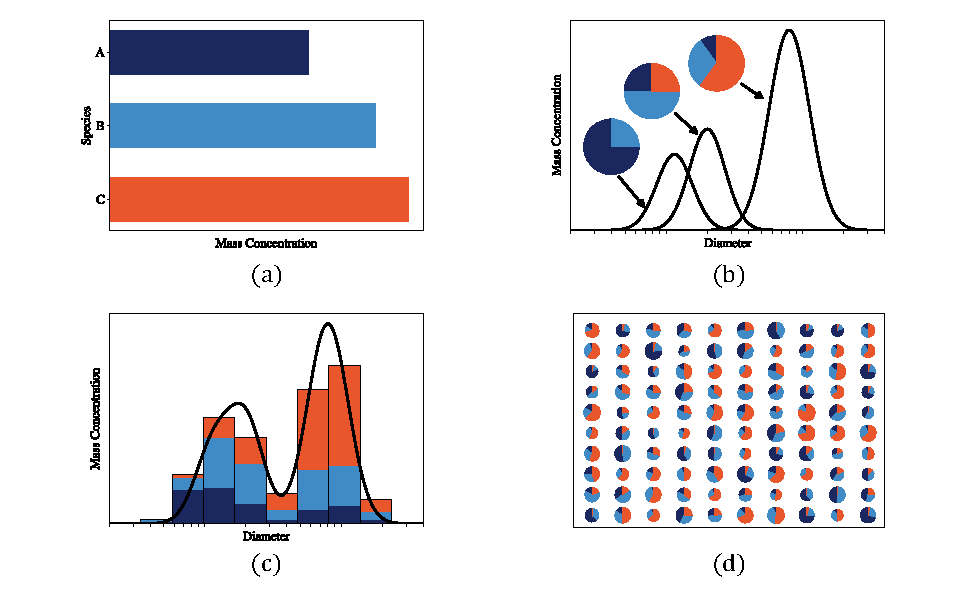
\includegraphics[width=\textwidth]{chapter1/aerosol-model-treatments.pdf}
	\caption{Cartoon representations of aerosol modeling treatments, each for the same aerosol population. The following representations are shown: (a) Bulk, (b) Modal, (c) 1-D sectional, (d) Particle-resolved.}
	\label{fig:test}
\end{figure}
